%% Week 36 -- Statistics, the bias-variance tradeoff and resampling methods
%% Sources: Sections 2.3-2.12 of chapter2.tex (expectation values, CLT,
%% estimators, statistics of OLS, training/test error, bias-variance,
%% bootstrap, cross-validation), with examples adapted from week38.do.txt.
%% The lecture opens with a lean reminder of OLS/Ridge/Lasso from week 35 and
%% the train/test U-curve (exercise3_train_test.pdf, made for week 35), which
%% motivates the bias-variance discussion.  The MLE derivation of OLS is a
%% bridge to the Bayesian reading of Ridge and Lasso planned for week 37.
%% Part 5 (added 2026-09-01) covers the new book Section 3.14: cross-validation
%% for Ridge and Lasso done properly -- the procedure, the factor n, the
%% one-standard-error rule, bootstrap vs cross-validation, stability selection,
%% nested CV -- and reuses the chapter-3 book figures cv_ridge_lasso.pdf and
%% cv_versus_bootstrap.pdf.
%% Figures week36_*.pdf are produced by make_week36_figures.py; the same code
%% appears verbatim in week36tuesday.ipynb.
%% Build:  pdflatex week36slides.tex  (twice)
\documentclass[10pt,aspectratio=169]{beamer}
\usetheme{red_plain}
\usepackage[T1]{fontenc}
\usepackage[utf8]{inputenc}
\usepackage{amsmath,amssymb,bm}
\usepackage{graphicx}
\usepackage{listings}
\usepackage{xcolor}
\usepackage{booktabs}
\graphicspath{{../BookFigures/chapter02_statistics/}{../BookFigures/chapter03_linear_regression/}{./}}

%% ---- code listings
\definecolor{codebg}{rgb}{0.97,0.97,0.97}
\lstset{language=Python,basicstyle=\ttfamily\scriptsize,backgroundcolor=\color{codebg},
  keywordstyle=\color{blue!70!black}\bfseries,commentstyle=\color{green!45!black},
  stringstyle=\color{red!60!black},showstringspaces=false,frame=single,
  framerule=0pt,xleftmargin=4pt,xrightmargin=4pt,breaklines=true,columns=fullflexible}

%% ---- the "pause and think" question frames
\newcounter{insight}
\newenvironment{insight}[1][]{%
  \stepcounter{insight}%
  \begin{frame}{Pause and think \arabic{insight}: #1}%
  \setbeamercolor{block title}{bg=structure.fg,fg=white}%
  \setbeamercolor{block body}{bg=structure.fg!8}%
}{\end{frame}}
\newcommand{\question}[1]{\begin{block}{Question}#1\end{block}}
\newcommand{\answer}[1]{\pause\begin{block}{Answer}#1\end{block}}
\newcommand{\hint}[1]{\pause{\small\emph{Hint: }#1}}

\setbeamertemplate{footline}[frame number]
\setbeamertemplate{blocks}[rounded][shadow=false]
\setbeamercovered{invisible}

\title{Week 36: The Bias--Variance Tradeoff and Resampling Methods}
\subtitle{Why the test error is U-shaped, and how to estimate it honestly\\[3pt]
  \small With pauses for questions}
\author{Morten Hjorth-Jensen}
\institute{Department of Physics and Center for Computing in Science Education,\\
  University of Oslo, Norway}
\date{}

\begin{document}

\begin{frame}
\titlepage
\end{frame}

\begin{frame}{Plan for week 36}
\textbf{Monday lecture (2$\times$45 min):}
\begin{itemize}
  \item A lean reminder of OLS, Ridge and Lasso from last week ($\sim$10--15 min)
  \item The training/test figure as function of polynomial degree -- the
        question this whole week answers
  \item The statistical toolbox (Sections 2.3--2.8): expectation values,
        sample estimators, the central limit theorem, and the statistics of
        the OLS and Ridge estimators
  \item Deriving the bias-variance tradeoff, Eq.~(2.52), with code
  \item Resampling methods: the bootstrap and $k$-fold cross-validation
  \item Cross-validation done properly for Ridge and Lasso (Section 3.14)
\end{itemize}
\vspace{4pt}
\textbf{Tuesday session (2$\times$45 min, flipped):} your questions, then two
cases -- the bias-variance decomposition by the bootstrap, and the full
cross-validation recipe for Ridge and Lasso.  Bring your laptop.
\vspace{4pt}
\begin{block}{Reading}
Chapter 2, Sections 2.3--2.12 and Chapter 3, Section 3.14 of the book.
Hastie et al., Sections 7.1--7.5, 7.10 (cross-validation) and 7.11
(bootstrap).  Every few slides there is a
\emph{Pause and think} frame: talk to your neighbour for a minute, then we
discuss.
\end{block}
\end{frame}

%% ====================================================================
%% Part 1 -- reminder from week 35
%% ====================================================================

\begin{frame}{Reminder from week 35: the three estimators in one view}
With the SVD $\bm{X}=\bm{U}\bm{\Sigma}\bm{V}^T$, ordinary least squares reads
\[
  \hat{\bm{\theta}}_{\mathrm{OLS}}
   = \left(\bm{X}^T\bm{X}\right)^{-1}\bm{X}^T\bm{y}
   = \sum_{i=0}^{p-1}\frac{\bm{u}_i^T\bm{y}}{\sigma_i}\,\bm{v}_i,
  \qquad
  \tilde{\bm{y}}_{\mathrm{OLS}} = \bm{U}\bm{U}^T\bm{y},
\]
Ridge regression changes the picture in exactly one place, multiplying each
mode by the shrinkage factor of Eq.~(3.48),
\[
  \hat{\bm{\theta}}_{\mathrm{Ridge}}
   = \sum_{i=0}^{p-1}\frac{\sigma_i^2}{\sigma_i^2+\lambda}\,
     \frac{\bm{u}_i^T\bm{y}}{\sigma_i}\,\bm{v}_i,
\]
and the Lasso replaces smooth shrinkage by soft thresholding,
Eq.~(3.63): coefficients are moved towards zero by $\lambda/2$ and clipped at
zero -- shrinkage \emph{and} selection.
\vspace{4pt}
\begin{block}{Last week's language}
We said: ``Ridge trades a little bias for a large reduction in variance.''
We used the words -- today we earn them.  Bias and variance \emph{of what},
with respect to \emph{which} randomness?
\end{block}
\end{frame}

\begin{frame}{Reminder from week 35: what the penalty does to the numbers}
For a singular value $\sigma_i$ of the design matrix:
\begin{itemize}
  \item \textbf{OLS} keeps the mode untouched: factor $1$.  Small $\sigma_i$
        (nearly collinear columns) amplify the data noise by $1/\sigma_i$.
  \item \textbf{Ridge} damps each mode by $\sigma_i^2/(\sigma_i^2+\lambda)$:
        modes with $\sigma_i^2\gg\lambda$ survive, modes with
        $\sigma_i^2\ll\lambda$ are suppressed.
  \item \textbf{Lasso} sets small coefficients exactly to zero (the corner of
        the $1$-norm ball from last week's geometry figure).
\end{itemize}
\vspace{6pt}
This week we make the statistical content of these statements precise, and we
meet the experimental tools -- resampling methods -- that let us \emph{measure}
bias and variance from a single data set.
\end{frame}

\begin{insight}[which estimator is unbiased?]
\question{One of the three estimators above satisfies
$\mathbb{E}[\hat{\bm{\theta}}]=\bm{\theta}$, the true parameters.  Which one,
and what assumption about the data does the statement silently rely on?}
\answer{OLS, Eq.~(2.45) -- \emph{provided} the data really come from
$\bm{y}=\bm{X}\bm{\theta}+\bm{\varepsilon}$ with zero-mean noise.  If the true
$f(\bm{x})$ is not in the span of our features, OLS is biased no matter how
much data we collect.  Ridge is biased for any $\lambda>0$:
$\mathbb{E}[\hat{\bm{\theta}}_{\mathrm{Ridge}}]
=(\bm{X}^T\bm{X}+\lambda\bm{I})^{-1}\bm{X}^T\bm{X}\,\bm{\theta}\neq\bm{\theta}$.}
\end{insight}

%% ====================================================================
%% Part 2 -- the driving figure
%% ====================================================================

\begin{frame}{The figure that drives this week}
\begin{columns}
\begin{column}{0.55\textwidth}

\includegraphics[width=\textwidth]{exercise3_train_test}
\end{column}
\begin{column}{0.43\textwidth}
\small
Training and test MSE against polynomial degree, from last week's exercise 3
(seed 2026, $n=100$).
\begin{itemize}
  \item The \textbf{training error} falls monotonically -- a degree-$(n-1)$
        polynomial would drive it to zero.
  \item The \textbf{test error} falls, reaches a broad minimum, and rises:
        the celebrated U-curve.
\end{itemize}
\textbf{This week's question:} what law of statistics forces the U-shape,
and how do we find its minimum when data are scarce?
\end{column}
\end{columns}
\vspace{4pt}
The answer is an identity, Eq.~(2.52), plus two experimental techniques: the
bootstrap and cross-validation.  To derive the identity we first need the
statistical toolbox of Sections 2.3--2.8.
\end{frame}

%% ====================================================================
%% Part 3 -- the statistical toolbox, Sections 2.3-2.8
%% ====================================================================

\begin{frame}{Toolbox 1: expectation values, moments and variance (Section 2.3)}
For a stochastic variable $X$ with PDF $p(x)$ and a function $h$,
\[
  \mathbb{E}[h] = \int h(x)\,p(x)\,dx
  \qquad \text{(Eq.~2.12; a sum in the discrete case).}
\]
The moments $\mathbb{E}[x^n]$ summarise $p$; the two we use constantly are the
\textbf{mean} $\mu=\mathbb{E}[x]$ and the \textbf{variance}, Eq.~(2.16),
\[
  \sigma_X^2 = \mathrm{Var}(X) = \mathbb{E}\left[(x-\mu)^2\right]
             = \mathbb{E}[x^2]-\left(\mathbb{E}[x]\right)^2,
\]
-- the mean of the square minus the square of the mean, worth memorising.
From linearity, Eq.~(2.17),
\[
  \mathbb{E}[aX+b]=a\,\mathbb{E}[X]+b,
  \qquad
  \mathrm{Var}(aX+b)=a^2\,\mathrm{Var}(X):
\]
the variance ignores shifts and scales \emph{quadratically} -- the reason a
feature in millimetres has $10^6$ times the variance of the same feature in
metres, and the reason scaling mattered so much last Tuesday.
\end{frame}

\begin{frame}{Toolbox 2: covariance and independence (Section 2.4)}
For two stochastic variables, Eqs.~(2.18) and (2.19),
\[
  \mathrm{Cov}(X_i,X_j)
   = \mathbb{E}\left[(x_i-\mu_i)(x_j-\mu_j)\right]
   = \mathbb{E}[x_ix_j]-\mathbb{E}[x_i]\,\mathbb{E}[x_j],
\]
with $\mathrm{Cov}(X_i,X_i)=\mathrm{Var}(X_i)$.  If $X_i$ and $X_j$ are
\textbf{independent}, the joint PDF factorises and the covariance vanishes,
Eq.~(2.20).
\vspace{4pt}
\begin{block}{The converse is false, and it matters}
Take $X$ symmetric about zero and $Y=X^2$: then $\mathrm{Cov}(X,Y)=0$ although
$Y$ is a function of $X$.  Covariance sees only \emph{linear} dependence.
\end{block}
\vspace{4pt}
Independence is the assumption hiding inside almost everything today: the
central limit theorem, the bootstrap and the random splits of
cross-validation all require it.  Keep asking: \emph{are my samples
independent?}
\end{frame}

\begin{frame}{Toolbox 3: samples and estimators (Section 2.6)}
In practice we never know $p(x)$; we have $n$ measurements.  From them we
build the \textbf{sample mean} and \textbf{sample variance}, Eq.~(2.25),
\[
  \bar{x}=\frac{1}{n}\sum_{k=0}^{n-1}x_k,
  \qquad
  s^2=\frac{1}{n-1}\sum_{k=0}^{n-1}(x_k-\bar{x})^2 .
\]
These are \textbf{estimators}: functions of the data that approximate
properties of the unknown distribution.
\vspace{4pt}
\begin{block}{The one idea to take home today}
An estimator is a function of random variables, so it is \emph{itself a random
variable}, with a distribution, a mean and a variance of its own.  Everything
that follows -- the bias-variance tradeoff, the bootstrap, cross-validation --
is about exploring that distribution.
\end{block}
\end{frame}

\begin{insight}[why $n-1$?]
\question{The sample variance in Eq.~(2.25) divides by $n-1$, yet the sample
mean divides by $n$.  Why the asymmetry?}
\answer{Using $\bar{x}$ instead of the unknown $\mu$ makes the squared
deviations systematically too small: $\bar{x}$ is precisely the value that
\emph{minimises} $\sum_k(x_k-c)^2$ for the sample at hand.  A short
calculation, Eq.~(2.28), gives
$\mathbb{E}[\frac{1}{n}\sum_k(x_k-\bar{x})^2]=\frac{n-1}{n}\sigma^2$: one
degree of freedom was spent estimating the mean, and dividing by $n-1$
(Bessel's correction) restores unbiasedness.  Same story behind the $n-p$ in
the residual variance of regression.}
\end{insight}

\begin{frame}{Toolbox 4: bias, variance and the MSE of an estimator (Section 2.6)}
Let $\hat{\theta}$ estimate a quantity $\theta$.  Its \textbf{bias} is the
systematic error, Eq.~(2.26),
$\mathrm{Bias}(\hat{\theta})=\mathbb{E}[\hat{\theta}]-\theta$; its
\textbf{variance} measures how much it moves when the sample is redrawn.
Adding and subtracting $\mathbb{E}[\hat{\theta}]$ in the mean squared error
gives Eq.~(2.27),
\[
  \boxed{\;
  \mathbb{E}\left[(\hat{\theta}-\theta)^2\right]
   = \underbrace{\left(\mathbb{E}[\hat{\theta}]-\theta\right)^2}_{\mathrm{Bias}^2}
   + \underbrace{\mathbb{E}\left[(\hat{\theta}-\mathbb{E}[\hat{\theta}])^2\right]}_{\mathrm{Var}(\hat{\theta})}
  \;}
\]
the cross term vanishing because
$\mathbb{E}\left[\hat{\theta}-\mathbb{E}[\hat{\theta}]\right]=0$.
\vspace{4pt}
\begin{block}{Why this innocent identity runs the whole week}
An unbiased estimator is not automatically a good one: a biased estimator
with much smaller variance can have the \emph{smaller total error}.  That is
the bargain Ridge offers.  The bias-variance tradeoff of Section 2.10 is this
identity applied to a \emph{prediction} instead of a parameter.
\end{block}
\end{frame}

\begin{frame}{Toolbox 5: the central limit theorem (Section 2.5)}
\begin{columns}
\begin{column}{0.52\textwidth}
Average $m$ independent draws from \emph{any} PDF $p(x)$ with mean $\mu$ and
finite variance $\sigma^2$, Eq.~(2.22):
\[
  z=\frac{x_0+x_1+\dots+x_{m-1}}{m}.
\]
Then as $m$ grows, $\tilde{p}(z)$ tends to a Gaussian with mean $\mu$ and
variance $\sigma^2/m$, whatever the shape of $p(x)$.  The practical statement
is the \textbf{standard error}, Eq.~(2.24),
\[
  \boxed{\;\sigma_m=\frac{\sigma}{\sqrt{m}}\;}
\]
Four times the data halves the uncertainty: large data sets help, and help
\emph{slowly}.
\end{column}
\begin{column}{0.46\textwidth}
\includegraphics[width=\textwidth]{central_limit_theorem}
{\scriptsize Uniform and exponential averages become Gaussian by $m\sim10$;
Cauchy averages never do -- no finite variance, no theorem.}
\end{column}
\end{columns}
\end{frame}

\begin{frame}{What the CLT promises -- and what it does not}
Two conditions, both routinely forgotten:
\begin{enumerate}
  \item \textbf{Finite variance.}  Heavy-tailed distributions (Cauchy) have
        none; their sample means never settle down.
  \item \textbf{Independence.}  For correlated data the standard error
        $\sigma/\sqrt{m}$ \emph{underestimates} the true uncertainty, often
        by a large factor (Section 2.7: the factor is the autocorrelation
        time $\tau$, and methods like blocking exist to repair it).
\end{enumerate}
\vspace{4pt}
\begin{block}{Machine learning connection}
Eq.~(2.24) is why a test set of $1000$ points pins the test error to roughly
$3\%$ relative accuracy -- and why comparing two models whose test errors
differ by less than that is meaningless.  It also underwrites the bootstrap
below, and explains why the gradient noise in stochastic gradient descent
scales as $1/\sqrt{B}$ with batch size $B$.
\end{block}
\end{frame}

\begin{insight}[error bars on the test error]
\question{You compare two regression models on the same test set of $n=1000$
points and find test MSEs of $0.100$ and $0.103$.  Is the first model better?}
\answer{You cannot tell.  The test MSE is itself a sample mean of $1000$
squared residuals, so it carries a standard error of order
$\sigma_{\mathrm{res}}/\sqrt{1000}\approx3\%$ of its value -- as large as the
difference.  You would need either a much larger test set or paired
comparisons across resampled splits (bootstrap or cross-validation, coming
up) before declaring a winner.}
\end{insight}

\begin{frame}{The statistics of the least-squares estimator (Section 2.8)}
Assume the data are generated by the linear model, Eqs.~(2.37) and (2.38),
\[
  \bm{y}=\bm{X}\bm{\theta}+\bm{\varepsilon},
  \qquad
  \varepsilon_i\sim\mathcal{N}(0,\sigma^2)\ \text{independent},
\]
so that, Eq.~(2.39), $\mathbb{E}[y_i]=\bm{X}_{i,*}\bm{\theta}$ and
$\mathrm{Var}(y_i)=\sigma^2$: the design matrix is fixed, all randomness
enters through the noise.  Then
\[
  \mathbb{E}[\hat{\bm{\theta}}]
   = (\bm{X}^T\bm{X})^{-1}\bm{X}^T\,\mathbb{E}[\bm{y}]
   = \bm{\theta}
  \qquad \text{(Eq.~2.40: OLS is unbiased)},
\]
and using
$\mathbb{E}[\bm{y}\bm{y}^T]=\bm{X}\bm{\theta}\bm{\theta}^T\bm{X}^T+\sigma^2\bm{I}$,
\[
  \boxed{\;\mathrm{Var}(\hat{\bm{\theta}})
   = \sigma^2\left(\bm{X}^T\bm{X}\right)^{-1}\;}
  \qquad \text{(Eq.~2.42)}.
\]
The standard error of coefficient $j$ is
$\sigma(\hat{\theta}_j)=\sigma\sqrt{[(\bm{X}^T\bm{X})^{-1}]_{jj}}$,
Eq.~(2.48) -- exactly what you need for the confidence intervals of this
week's exercises, with $\hat{\sigma}^2=\|\bm{y}-\bm{X}\hat{\bm{\theta}}\|_2^2/(n-p)$.
\end{frame}

\begin{frame}{The same statistics for Ridge}
Repeating the computation for the Ridge estimator gives
\[
  \mathbb{E}\big[\hat{\bm{\theta}}_{\mathrm{Ridge}}\big]
   = (\bm{X}^T\bm{X}+\lambda\bm{I}_{pp})^{-1}(\bm{X}^T\bm{X})\,\bm{\theta}
   \neq \bm{\theta} \quad (\lambda>0):
  \qquad \text{biased,}
\]
\[
  \mathrm{Var}\big[\hat{\bm{\theta}}_{\mathrm{Ridge}}\big]
   = \sigma^2\,[\bm{X}^T\bm{X}+\lambda\bm{I}]^{-1}\bm{X}^T\bm{X}\,
     \big([\bm{X}^T\bm{X}+\lambda\bm{I}]^{-1}\big)^T
   \;\xrightarrow{\;\lambda\to\infty\;}\;0 .
\]
The difference is non-negative definite,
\[
  \mathrm{Var}[\hat{\bm{\theta}}_{\mathrm{OLS}}]
  -\mathrm{Var}[\hat{\bm{\theta}}_{\mathrm{Ridge}}]
   = \sigma^2[\bm{X}^T\bm{X}+\lambda\bm{I}]^{-1}
     \left[2\lambda\bm{I}+\lambda^2(\bm{X}^T\bm{X})^{-1}\right]
     \big([\bm{X}^T\bm{X}+\lambda\bm{I}]^{-1}\big)^T \succeq 0,
\]
so \textbf{for every} $\lambda>0$ Ridge has strictly smaller variance than
OLS.  Whether the trade is worth it is exactly the question Eq.~(2.27)
answers: it is, whenever the squared bias introduced is smaller than the
variance removed.
\end{frame}

\begin{insight}[read Eq.~(2.47) through the SVD]
\question{With $\bm{X}=\bm{U}\bm{\Sigma}\bm{V}^T$ we have
$(\bm{X}^T\bm{X})^{-1}=\bm{V}\tilde{\bm{\Sigma}}^{-2}\bm{V}^T$, so the
variance of $\hat{\bm{\theta}}$ along singular direction $i$ is
$\sigma^2/\sigma_i^2$.  What does a small singular value do, and what does
Ridge do about it?}
\answer{A nearly collinear pair of features means a small $\sigma_i$ and an
\emph{enormous} variance $\sigma^2/\sigma_i^2$ in that direction: the data
cannot determine the parameter.  The numerical ill-conditioning of week 34
and the statistical variance blow-up are the same fact in two languages.
Ridge multiplies each mode by $\sigma_i^2/(\sigma_i^2+\lambda)$, taming
exactly the directions that misbehave -- the promised variance reduction,
mode by mode.}
\end{insight}

%% ====================================================================
%% Part 3b -- MLE bridge
%% ====================================================================

\begin{frame}{Where does the squared cost come from?  OLS as maximum likelihood}
With Gaussian noise, a single output is distributed as
\[
  p(y_i,\bm{X}\vert\bm{\theta})
   = \frac{1}{\sqrt{2\pi\sigma^2}}
     \exp\left[-\frac{(y_i-\bm{X}_{i,*}\bm{\theta})^2}{2\sigma^2}\right],
\]
and for independent, identically distributed events the likelihood of the
whole data set $\bm{D}$ is the product
\[
  p(\bm{D}\vert\bm{\theta})
   = \prod_{i=0}^{n-1}p(y_i,\bm{X}\vert\bm{\theta}).
\]
\textbf{Maximum likelihood}: choose $\bm{\theta}$ so that the observed data
are the most probable.  Products of small numbers underflow and are painful to
differentiate, so we minimise the \emph{negative log-likelihood} instead --
the logarithm is monotonic, the optimum does not move.
\end{frame}

\begin{frame}{The negative log-likelihood is the OLS cost}
\[
  C(\bm{\theta})
   = -\log p(\bm{D}\vert\bm{\theta})
   = \frac{n}{2}\log(2\pi\sigma^2)
     + \frac{\|\bm{y}-\bm{X}\bm{\theta}\|_2^2}{2\sigma^2}.
\]
The first term is a constant; minimising $C$ is minimising the mean squared
error.  Setting the gradient to zero,
\[
  \bm{X}^T(\bm{y}-\bm{X}\bm{\theta})=0
  \quad\Longrightarrow\quad
  \hat{\bm{\theta}}_{\mathrm{OLS}}=(\bm{X}^T\bm{X})^{-1}\bm{X}^T\bm{y}.
\]
\vspace{2pt}
\begin{block}{Why show this now}
The squared cost is not an aesthetic choice: it \emph{is} the Gaussian noise
assumption.  Next week we put a prior on $\bm{\theta}$ and rerun the same
argument -- a Gaussian prior will hand us Ridge, a Laplace prior the Lasso.
\end{block}
\end{frame}

%% ====================================================================
%% Part 4 -- the bias-variance tradeoff
%% ====================================================================

\begin{frame}{The bias-variance tradeoff: the setup (Section 2.10)}
The data are generated by a noisy process, Eq.~(2.49),
\[
  \bm{y}=f(\bm{x})+\bm{\varepsilon},
  \qquad
  \bm{\varepsilon}\sim\mathcal{N}(0,\sigma^2),
\]
with $f$ unknown.  We fit a model on a training set and obtain predictions
$\tilde{\bm{y}}$; the cost we decompose is Eq.~(2.50),
\[
  \mathbb{E}\left[(\bm{y}-\tilde{\bm{y}})^2\right]
   = \frac{1}{n}\sum_{i=0}^{n-1}(y_i-\tilde{y}_i)^2 .
\]
\begin{block}{The essential point -- and the source of most confusion}
The expectation runs over \textbf{two} sources of randomness: the noise
$\bm{\varepsilon}$ \emph{and the training set itself}.  The model
$\tilde{\bm{y}}$ is a random variable because the data it was fitted to were
random: redraw the training set and the fitted polynomial moves.
$\mathbb{E}[\tilde{\bm{y}}]$ is the \emph{average prediction over training
sets}.
\end{block}
\end{frame}

\begin{frame}{The derivation, step by step}
Insert $\bm{y}=\bm{f}+\bm{\varepsilon}$ and add and subtract
$\mathbb{E}[\tilde{\bm{y}}]$, Eq.~(2.51),
\[
  \mathbb{E}\left[(\bm{y}-\tilde{\bm{y}})^2\right]
   = \mathbb{E}\left[\left(\bm{f}+\bm{\varepsilon}-\tilde{\bm{y}}
     +\mathbb{E}[\tilde{\bm{y}}]-\mathbb{E}[\tilde{\bm{y}}]\right)^2\right].
\]
Expanding gives three squared terms and three cross terms.  Every cross term
dies:
\begin{itemize}
  \item terms linear in $\bm{\varepsilon}$: the noise has zero mean and is
        independent of the training set;
  \item the remaining term: $\mathbb{E}\left[\tilde{\bm{y}}
        -\mathbb{E}[\tilde{\bm{y}}]\right]=0$, while $\bm{f}$ and
        $\mathbb{E}[\tilde{\bm{y}}]$ are not stochastic.
\end{itemize}
What survives is Eq.~(2.52):
\[
  \boxed{\;
  \mathbb{E}\left[(\bm{y}-\tilde{\bm{y}})^2\right]
   = \underbrace{\frac{1}{n}\sum_i\left(f_i-\mathbb{E}[\tilde{\bm{y}}]\right)^2}_{\mathrm{Bias}^2}
   + \underbrace{\frac{1}{n}\sum_i\left(\tilde{y}_i-\mathbb{E}[\tilde{\bm{y}}]\right)^2}_{\mathrm{Var}[\tilde{\bm{y}}]}
   + \;\sigma^2
  \;}
\]
-- Eq.~(2.27) again, applied to a prediction instead of a parameter.
\end{frame}

\begin{frame}{Reading the three terms}
\begin{description}
  \item[Bias$^2$] How far the \emph{average} prediction is from the truth:
        the error built into the model's simplifying assumptions.  A straight
        line through curved data has large bias, and no amount of data
        removes it.  \emph{Decreases} with model complexity.
  \item[Variance] How much the prediction moves when the training set is
        redrawn.  A flexible model chases the noise of whatever sample it
        got, so its predictions differ wildly between training sets.
        \emph{Increases} with model complexity.
  \item[$\sigma^2$] The irreducible error: no model can predict the noise
        term.  A hard floor under the test error.
\end{description}
\vspace{4pt}
The test error is their sum: it falls while the bias falls, then rises when
the variance takes over -- \textbf{the U-curve of the opening figure is
Eq.~(2.52) in action}.  Model selection is the business of locating the
minimum.
\end{frame}

\begin{insight}[a suspiciously good model]
\question{A fellow student reports a test MSE \emph{below} your best estimate
of the noise level $\sigma^2$.  Brilliant model or a bug?}
\answer{A bug (or leakage).  By Eq.~(2.52) the expected test error can never
lie below $\sigma^2$: no model predicts noise.  A test error at or under the
noise floor means test data leaked into training or preprocessing, the noise
estimate is wrong, or the test set is too small for its own error bar
(Pause and think 3).  Healthy scepticism about ``too good'' numbers is a
transferable skill.}
\end{insight}

\begin{frame}[fragile]{Estimating the three terms: the bootstrap manufactures the ensemble}
Eq.~(2.52) wants an average over training sets -- but we have \emph{one} data
set.  The bootstrap (details in a moment) fakes the ensemble by resampling
the training data with replacement:
\begin{lstlisting}
np.random.seed(2026)
n, n_bootstraps, maxdegree = 40, 100, 14
x = np.linspace(-3, 3, n).reshape(-1, 1)
y = np.exp(-x**2) + 1.5*np.exp(-(x - 2)**2) + np.random.normal(0, 0.1, x.shape)
x_train, x_test, y_train, y_test = train_test_split(x, y, test_size=0.2,
                                                    random_state=2026)
for degree in range(maxdegree):
    model = make_pipeline(PolynomialFeatures(degree=degree),
                          LinearRegression(fit_intercept=False))
    y_pred = np.empty((y_test.shape[0], n_bootstraps))
    for i in range(n_bootstraps):
        x_, y_ = resample(x_train, y_train)                # draw with replacement
        y_pred[:, i] = model.fit(x_, y_).predict(x_test).ravel()
    error[degree]    = np.mean(np.mean((y_test - y_pred)**2, axis=1, keepdims=True))
    bias[degree]     = np.mean((y_test - np.mean(y_pred, axis=1, keepdims=True))**2)
    variance[degree] = np.mean(np.var(y_pred, axis=1, keepdims=True))
\end{lstlisting}
Averages along \lstinline{axis=1} are expectations over training sets;
\lstinline{keepdims=True} keeps the column shape and is essential for the bias
to come out right (drop it and enjoy the debugging).
\end{frame}

\begin{frame}{The decomposition, measured}
\begin{columns}
\begin{column}{0.55\textwidth}
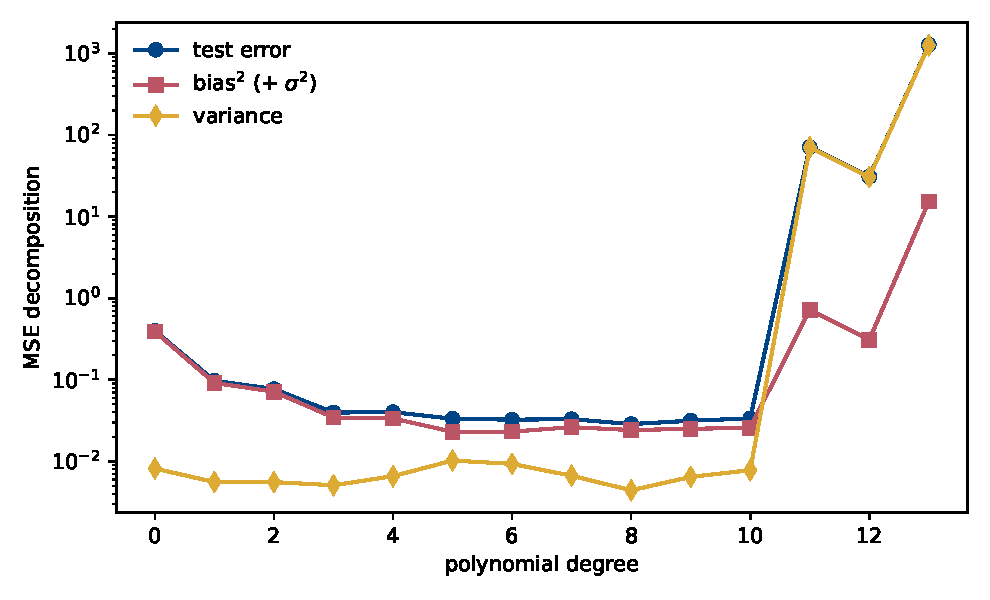
\includegraphics[width=\textwidth]{week36_bias_variance}
\end{column}
\begin{column}{0.43\textwidth}
\small
Seed 2026, $n=40$, 100 bootstraps (Tuesday's Case 1).
\begin{itemize}
  \item Bias$^2$ falls from $0.39$ at degree 0 to $\approx0.02$ by degree 5
        and flattens: the polynomial family is then rich enough.
  \item Variance is negligible up to degree $\sim$10, then explodes
        ($0.008\to10^3$).
  \item The sum has a broad minimum around degrees 5--9.
\end{itemize}
Because we compare with $y_{\mathrm{test}}$ rather than the unknown $f$, the
measured ``bias'' absorbs $\sigma^2=0.01$ -- its floor sits just above the
true squared bias.
\end{column}
\end{columns}
\end{frame}

\begin{insight}[equality or inequality?]
\question{The code prints \texttt{error >= bias + variance}.  Our derivation
of Eq.~(2.52) produced an \emph{equality}.  Who is lying?}
\answer{Nobody.  The derivation's bias compares
$\mathbb{E}[\tilde{\bm{y}}]$ with the true $f$, which the code does not know;
it uses $y_{\mathrm{test}}=f+\varepsilon$ instead.  The measured bias term
therefore contains the irreducible $\sigma^2$, and the printed identity holds
as an equality only in expectation, with finite-sample noise on top.  Knowing
exactly \emph{which} quantity your code estimates is half of statistics.}
\end{insight}

\begin{frame}{Every regularisation method is a move on this curve}
\begin{itemize}
  \item \textbf{Ridge and Lasso} add bias to remove variance -- now a theorem
        (the variance difference above), not a slogan.
  \item \textbf{Early stopping} halts training before the variance grows.
  \item \textbf{Bagging and random forests} average many high-variance models
        to cancel variance; \textbf{boosting} combines many high-bias models
        to reduce bias.
  \item \textbf{Dropout, data augmentation}: variance reduction in neural
        networks.
\end{itemize}
Knowing which of the two terms a method attacks predicts whether it will help.
\vspace{4pt}
\begin{block}{A modern caveat}
The clean U-shape is a statement about models of moderate capacity.  Heavily
overparameterised networks show \emph{double descent}: past the interpolation
threshold the test error can fall again.  We return to this in the neural
network chapters.
\end{block}
\end{frame}

%% ====================================================================
%% Part 5 -- resampling: the bootstrap
%% ====================================================================

\begin{frame}{Why resampling methods?}
In our eagerness to fit, we omitted the questions that matter:
\begin{itemize}
  \item How uncertain is an estimated quantity -- a parameter, a test error?
  \item How do we \emph{measure} bias and variance with one finite data set?
  \item How do we select a model without wasting data?
\end{itemize}
\textbf{Resampling}: repeatedly draw samples from the training data, refit
the model on each, and study how the results vary.  Computationally greedy --
we fit the same model hundreds of times -- and, with today's computers,
routinely affordable.
\vspace{4pt}
The two workhorses of machine learning, both used in Project 1:
\begin{enumerate}
  \item the \textbf{bootstrap} (model assessment: distributions and error
        bars for estimators);
  \item \textbf{cross-validation} (model selection: choosing degree,
        $\lambda$, \dots).
\end{enumerate}
Relatives: the jackknife (leave-one-out, Section 2.11) and blocking for
correlated data (Section 2.7).
\end{frame}

\begin{frame}{The bootstrap: Efron's idea (Section 2.11)}
$\hat{\theta}=\hat{\theta}(\bm{X})$ is a random variable with some unknown PDF
$p(t)$.  If we knew the data-generating $p(x)$ we could learn $p(t)$ by brute
force: draw fresh samples, recompute $\hat{\theta}$, histogram.  We do not
know $p(x)$.
\vspace{4pt}
\begin{block}{Efron (1979)}
Replace $p(x)$ by the \emph{empirical} distribution of the observed data.
Drawing from it is simply drawing the observed values \textbf{with
replacement} -- and asymptotically this recovers the right answer.
\end{block}
\vspace{4pt}
\textbf{The algorithm:}
\begin{enumerate}
  \item Draw with replacement $n$ values from $\bm{x}=(x_0,\dots,x_{n-1})$,
        forming the resample $\bm{x}^*$.
  \item Compute the replica $\hat{\theta}^*=\hat{\theta}(\bm{x}^*)$.
  \item Repeat $k$ times; the spread of the replicas estimates the
        distribution of $\hat{\theta}$.
\end{enumerate}
No Gaussian assumption, works for statistics with no known formula (a median,
a ratio, a test error), and often beats asymptotic formulae for small samples.
It \emph{requires} iid data -- for correlated data use block bootstrap.
\end{frame}

\begin{frame}[fragile]{The bootstrap at work, checked against the CLT}
\begin{columns}
\begin{column}{0.5\textwidth}
\begin{lstlisting}
def bootstrap(data, statistic, k=1000, rng=None):
    rng = np.random.default_rng() if rng is None else rng
    n = len(data)
    replicas = np.empty(k)
    for i in range(k):
        sample = data[rng.integers(0, n, n)]
        replicas[i] = statistic(sample)
    return replicas

rng = np.random.default_rng(2026)
x = rng.normal(100.0, 15.0, 10000)
t = bootstrap(x, np.mean, k=1000, rng=rng)
\end{lstlisting}
{\small The bootstrap standard error is $0.1523$; the CLT prediction
$\sigma/\sqrt{n}=0.1508$.  For the mean of iid data the CLT already knew the
answer -- the value of the bootstrap is that the code keeps working when
\lstinline{np.mean} is replaced by any statistic.}
\end{column}
\begin{column}{0.48\textwidth}
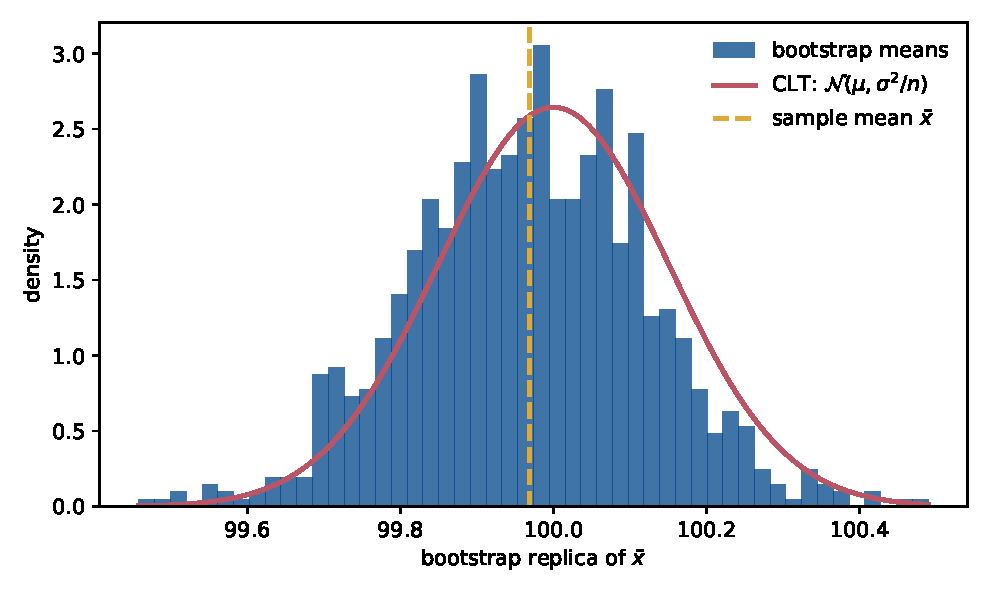
\includegraphics[width=\textwidth]{week36_bootstrap_hist}
\end{column}
\end{columns}
\end{frame}

\begin{insight}[why with replacement?]
\question{Why must the bootstrap draw \emph{with} replacement?  What would $k$
draws \emph{without} replacement of size $n$ give?}
\answer{Without replacement, every resample of size $n$ is the original data
set in a different order: every replica $\hat{\theta}^*$ is identical and the
estimated variance is exactly zero.  Drawing with replacement makes each
resample a genuine draw from the empirical distribution -- on average
$1-1/e\approx63\%$ of the original points appear, some repeated -- so the
replicas scatter the way $\hat{\theta}$ would across real repeated
experiments.}
\end{insight}

%% ====================================================================
%% Part 6 -- cross-validation
%% ====================================================================

\begin{frame}{Cross-validation: structuring the split (Section 2.12)}
A single train/test split wastes data, and the answer depends on which points
landed where.  Random re-splitting helps but leaves some points
over-represented.  \textbf{$k$-fold cross-validation} removes the imbalance:
\begin{enumerate}
  \item Shuffle the data set at random.
  \item Split it into $k$ roughly equal, mutually exclusive folds.
  \item Each fold in turn is the test set; fit on the other $k-1$ folds,
        evaluate on the held-out fold, record the score, discard the model.
  \item Summarise by the mean -- and the spread -- of the $k$ scores.
\end{enumerate}
Every observation is tested exactly once and trained on exactly $k-1$ times.
\vspace{4pt}
$k=n$ is \textbf{leave-one-out} (LOOCV): the jackknife of Eq.~(2.53) applied
to prediction error.  Unbiased but expensive ($n$ fits) and high-variance
(the $n$ training sets are nearly identical).  $k$ between 5 and 10 is the
usual compromise.
\end{frame}

\begin{insight}[choosing $k$]
\question{Your data set has $n=10^6$ points and one model fit takes a minute.
Do you use LOOCV?  And on $n=50$ points?}
\answer{Never at $n=10^6$: a million fits, and the tiny variance gain is
worthless anyway -- with that much data even a single split is accurate (CLT
again).  At $n=50$, data are precious: LOOCV (50 quick fits) or $k=10$ is
sensible, and the spread across folds gives the error bar the single split
could not.  The right $k$ is a cost/benefit decision, not a constant of
nature.}
\end{insight}

\begin{frame}{The standard use: selecting the Ridge penalty}
For each $\lambda$ on a (logarithmic) grid, and each fold $i$, fit on the data
with fold $i$ removed, Eq.~(2.54),
\[
  \bm{\theta}_{-i}(\lambda)
   = \left(\bm{X}_{-i,*}^T\bm{X}_{-i,*}+\lambda\bm{I}_{pp}\right)^{-1}
     \bm{X}_{-i,*}^T\,\bm{y}_{-i},
\]
evaluate the MSE on fold $i$, and average over folds.  Choose the $\lambda$
minimising the cross-validated error; refit on all data.
\vspace{4pt}
The same recipe selects the polynomial degree, the Lasso penalty, a learning
rate, a network width -- \textbf{cross-validation is the universal knob-tuner
of this course}.  The one iron rule: the test set proper is touched exactly
once, at the very end; $\lambda$ is chosen on the folds, never on the final
test data.
\end{frame}

\begin{frame}[fragile]{Code: own KFold loop vs \texttt{cross\_val\_score}}
\begin{lstlisting}
rng = np.random.default_rng(2026)
x = rng.standard_normal(100)
y = 3*x**2 + rng.standard_normal(100)          # noise variance is 1

lambdas = np.logspace(-3, 5, 100)
kfold = KFold(n_splits=5, shuffle=True, random_state=2026)

# own loop: scaler and Ridge fitted on the training folds only
for i, lmb in enumerate(lambdas):
    for j, (train_inds, test_inds) in enumerate(kfold.split(x)):
        Xtrain = poly.fit_transform(x[train_inds][:, np.newaxis])
        Xtest  = poly.transform(x[test_inds][:, np.newaxis])
        scaler = StandardScaler().fit(Xtrain)
        ridge  = Ridge(alpha=lmb).fit(scaler.transform(Xtrain), y[train_inds])
        ypred  = ridge.predict(scaler.transform(Xtest))
        scores_KFold[i, j] = np.mean((ypred - y[test_inds])**2)

# the same in three lines
pipe = make_pipeline(PolynomialFeatures(degree=6), StandardScaler(), Ridge(alpha=lmb))
scores = cross_val_score(pipe, x[:, np.newaxis], y, cv=kfold,
                         scoring="neg_mean_squared_error")
\end{lstlisting}
\end{frame}

\begin{frame}{Reading the cross-validation curve}
\begin{columns}
\begin{column}{0.55\textwidth}
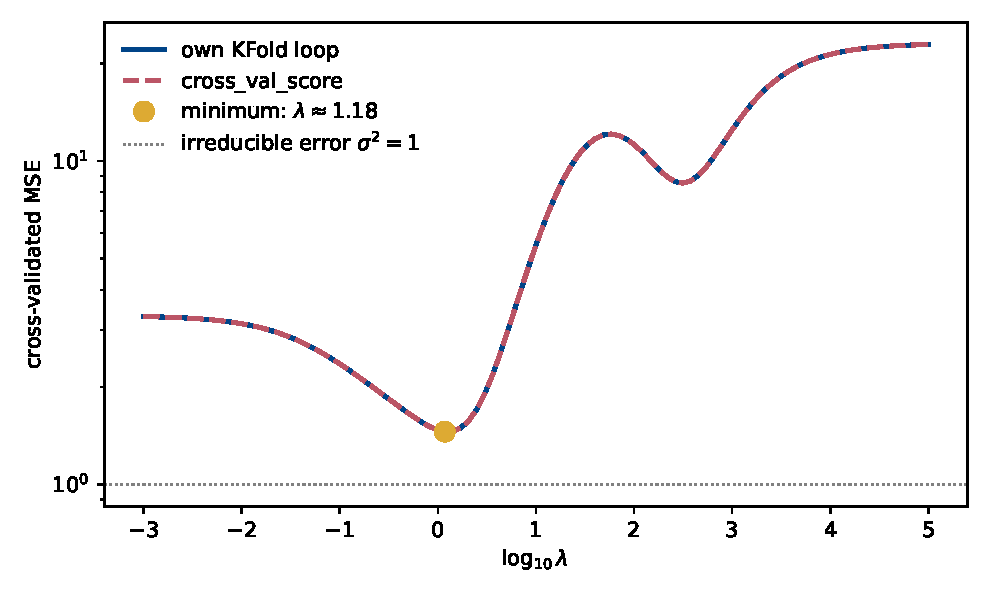
\includegraphics[width=\textwidth]{week36_cv_ridge}
\end{column}
\begin{column}{0.43\textwidth}
\small
Degree-6 polynomial on $y=3x^2+\varepsilon$, $n=100$, 5 folds (Tuesday's
Case 2).
\begin{itemize}
  \item The two curves lie on top of each other: \texttt{cross\_val\_score}
        does nothing magical.
  \item The minimum sits near $\lambda\approx1$ with CV-MSE $\approx1.5$,
        hovering just above the irreducible $\sigma^2=1$ -- the method has
        recovered the noise floor from 100 points.
  \item At $\lambda=10^5$ every coefficient is crushed: the model predicts
        the mean and the error climbs to $\mathrm{Var}(y)$.
\end{itemize}
\end{column}
\end{columns}
\vspace{4pt}
The \texttt{StandardScaler} \emph{inside} the fold loop is not decoration: a
degree-6 basis has columns differing by orders of magnitude, and without
scaling the curve tails are numerical noise.
\end{frame}

\begin{insight}[the subtle leak]
\question{A pipeline scales the full data set \emph{once}, then runs 5-fold
cross-validation on the scaled data.  The CV error comes out slightly -- but
systematically -- too optimistic.  Why?}
\answer{The scaler's mean and variance were computed on \emph{all} the data,
so each training fold has already seen statistics of its own test fold: a
leak.  Small here, large when features are many.  Rule: \textbf{every}
preprocessing step that learns from data -- centring, scaling, feature
selection, PCA, imputation -- goes \emph{inside} the loop, refitted per fold.
In \texttt{scikit-learn}: wrap it in a \texttt{Pipeline} and cross-validate
the pipeline.  The same discipline applies to the bootstrap.}
\end{insight}

%% ====================================================================
%% Part 5 -- choosing the penalty properly (book Section 3.14)
%% ====================================================================

\begin{frame}{Doing it properly: cross-validation for Ridge and Lasso (Section 3.14)}
The recipe of the last frames is the outline.  The details are where the
mistakes live, and Section~3.14 of the book spells them out.  Start with the
distinction that makes cross-validation necessary at all:
\begin{itemize}
  \item \textbf{Model parameters} $\theta_0,\bm{\theta}$: fixed, at given
        $\lambda$, by minimising the cost.
  \item \textbf{Hyperparameter} $\lambda$: cannot be fixed the same way.  The
        unpenalised fit minimises the training error over \emph{all}
        $\bm{\theta}$, so for every $\lambda>0$
        \[
          \mathrm{Err}_{\mathrm{Train}}(\lambda)\;\ge\;\mathrm{Err}_{\mathrm{Train}}(0),
          \qquad\text{Eq.~(3.91)},
        \]
        and the training error is in fact non-decreasing along the whole
        path.  Minimising it over $\lambda$ always returns $\lambda=0$.
\end{itemize}
\vspace{2pt}
\begin{block}{Three errors, three roles}
The \textbf{training error} is minimised to get the parameters at fixed
$\lambda$; the \textbf{cross-validation error} is minimised over $\lambda$
to get the hyperparameter; the \textbf{test error} is computed once, at the
end, and minimised over nothing.
\end{block}
\end{frame}

\begin{frame}{The procedure, precisely}
Assign each of the $n$ training points to a fold, $\kappa(i)\in\{1,\dots,K\}$,
after a shuffle.  With $\hat{\theta}_0^{(-k)}(\lambda),\hat{\bm{\theta}}^{(-k)}(\lambda)$
fitted -- \emph{scaler included} -- to the points not in fold $k$,
\[
  \mathrm{CV}_K(\lambda)
   = \frac{1}{n}\sum_{i=0}^{n-1}
     \Bigl(y_i-\hat{\theta}_0^{(-\kappa(i))}(\lambda)
       -\bm{x}_i^T\hat{\bm{\theta}}^{(-\kappa(i))}(\lambda)\Bigr)^2
   = \frac{1}{K}\sum_{k=1}^{K}\mathrm{MSE}_k(\lambda),
  \qquad\text{Eq.~(3.92)},
\]
every point predicted once, by the model that did not see it.  The spread of
the $K$ fold errors gives a standard error, Eq.~(3.93),
\[
  \mathrm{SE}_K(\lambda)=\frac{1}{\sqrt{K}}\,\mathrm{std}\bigl(\mathrm{MSE}_1,\dots,\mathrm{MSE}_K\bigr)
\]
-- a rough guide, not a confidence interval: the $K$ training sets overlap,
so the fold errors are correlated.  Then
$\lambda_{\min}=\arg\min_\lambda\mathrm{CV}_K(\lambda)$, Eq.~(3.94).
\vspace{2pt}
\begin{block}{The two steps people forget}
\textbf{Refit:} the $K$ sets of fold coefficients were temporary -- the final
model is a \emph{new} fit at $\lambda_{\min}$ to all $n$ training points,
scaler refitted on all $n$.  \textbf{Test once:} only then, and only once, the
test set.  Report $\lambda$, the coefficients, CV $\pm$ SE, and the test error.
\end{block}
\end{frame}

\begin{frame}{Which $\lambda$ is being compared?  The factor $n$}
The fold models see $n(K-1)/K$ points, the final one $n$.  Is the same
numerical $\lambda$ the same penalty?  Depends on the convention.
\[
  \tfrac{1}{n}\|\bm{y}-\bm{X}\bm{\theta}\|_2^2+\lambda\|\bm{\theta}\|_2^2
  \;\Rightarrow\;
  \hat{\bm{\theta}}=(\bm{X}^T\bm{X}+n\lambda\bm{I})^{-1}\bm{X}^T\bm{y}
  \qquad\text{Eq.~(3.95)}
\]
$\bm{X}^T\bm{X}$ grows like $n$ (sums of $n$ products), and so does
$n\lambda$: $\lambda$ is a penalty \emph{per observation} and transfers from
80-point folds to the 100-point refit.  Without the $1/n$ -- Eq.~(3.44),
$(\bm{X}^T\bm{X}+\lambda\bm{I})^{-1}$ -- the same $\lambda$ is weaker by
$(K-1)/K$ on the full set.  One grid step; harmless; but know where it enters.
\vspace{3pt}
\begin{block}{The library conventions (Section 3.10 again)}
\texttt{scikit-learn}'s \texttt{Ridge}: no $1/n$, so \texttt{alpha} $=n\lambda$.
Its \texttt{Lasso}: $\|\cdot\|^2/(2n)+\alpha\|\bm{\theta}\|_1$, so
\texttt{alpha} $=\lambda/2$.  Same library, two conventions.  The
book keeps the $1/n$ of Eqs.~(3.43) and (3.57) throughout Section~3.14, and
so should your own code.
\end{block}
\vspace{2pt}
\small
\textbf{The grid:} logarithmic.  Lasso: from $\lambda_{\max}=\tfrac{2}{n}\|\bm{X}^T\bm{y}\|_\infty$
(Eq.~(3.67), above which everything is zero) down three or four decades, warm
starts on the way.  Ridge: for standardised columns the natural unit is
$\lambda\sim1$; $10^{-4}$ to $10$ covers every regime.  A minimum at the end
of the grid means the grid was wrong.
\end{frame}

\begin{frame}{The one-standard-error rule}
Near its minimum the CV curve is \emph{flat}, and the minimum is located only
to within the noise.  Among penalties the folds cannot tell apart, take the
most regularised:
\[
  \lambda_{1\mathrm{SE}}
   = \max\Bigl\{\lambda:\;\mathrm{CV}_K(\lambda)\le
       \mathrm{CV}_K(\lambda_{\min})+\mathrm{SE}_K(\lambda_{\min})\Bigr\},
  \qquad\text{Eq.~(3.96)}.
\]
\begin{itemize}
  \item For Ridge: a little more bias the data cannot detect, for a smaller
        variance.
  \item For the Lasso: a \emph{sparser} model -- which is usually why one
        uses the Lasso at all.
  \item A convention, not a theorem: the improvement of the more complex
        model is not larger than the uncertainty with which it is measured,
        so it is not believed.
\end{itemize}
\vspace{3pt}
\begin{block}{How unstable is $\lambda_{\min}$?}
Book Section~3.14, twenty different shuffles of the same 100 training points:
$\lambda_{\min}$ moves by a factor 5 for Ridge and by more than an order of
magnitude for the Lasso, taking the Lasso's support with it.  The prediction
is stable; the hyperparameter and the selected variables are not.  Remedies:
repeated CV (costly), the one-SE rule (cheap), and the bootstrap (next).
\end{block}
\end{frame}

\begin{insight}[the second decimal of $\lambda_{\min}$]
\question{Two students run 5-fold CV for Ridge on the same 100 points with
different shuffles and report $\lambda_{\min}=0.003$ and $0.013$.  Who is
right, and does it matter?}
\answer{Both, and mostly no.  The CV curve is flat along that whole valley:
its width there is smaller than the standard error, so the folds cannot rank
the two values, and the test errors of the two refitted models differ by
about a tenth.  What \emph{does} change is the fitted model -- and for the
Lasso, which variables it keeps.  Report $\lambda_{\min}$ with its
\emph{range}, or use the one-SE rule, which moves the choice onto the rising
flank where the curve determines its own position.}
\end{insight}

\begin{frame}{Ridge and Lasso side by side: a sparse truth (book Figure 3.4)}
\begin{columns}
\begin{column}{0.62\textwidth}

\includegraphics[width=\textwidth]{cv_ridge_lasso}
\end{column}
\begin{column}{0.37\textwidth}
\footnotesize
$p=30$ correlated features (corr.\ $0.7^{|i-j|}$), 8 true non-zeros,
$\sigma=1$, 100 training points.  Dashed: the \emph{true} test error of the
refit (20\,000 fresh points -- never available in practice).
\begin{itemize}
  \item Training error (dotted): monotone in $\lambda$, far below the test
        error -- it can select nothing.
  \item Ridge: $\lambda_{\min}=0.013$, true optimum $0.024$; the true errors
        differ by $0.02$.  Choice costs nothing.
  \item Lasso: $\lambda_{\min}$ hits the true optimum; true error $1.15$
        vs Ridge $1.29$ -- the truth is sparse, the Laplace prior is right.
  \item But the Lasso keeps 21 of 30 (8 true + 13 spurious): CV optimises
        \emph{prediction}, and small false coefficients cost nothing.  The
        one-SE choice keeps 13, all 8 true ones still in, at $1.28$.
\end{itemize}
\end{column}
\end{columns}
\end{frame}

\begin{insight}[a test set of fifty points]
\question{The book's run reports test errors $1.37$, $1.14$, $1.06$, $1.14$
for the four selected models, from a 50-point test set.  Does the one-SE
Ridge really beat the min-CV Ridge by $0.23$?}
\answer{No.  A mean squared error from $m=50$ residuals is itself an estimate;
for Gaussian residuals the squared residuals have variance $2\,\mathrm{MSE}^2$,
so Eq.~(2.24) gives a standard error of about $\mathrm{MSE}\sqrt{2/50}\approx0.2$.
The honest summary is ``all four generalise at about $1.2\pm0.2$, above the
floor of 1'' -- a test set of fifty cannot resolve tenths.  This is the
error-bar-on-the-test-error point from earlier today, now with teeth.}
\end{insight}

\begin{frame}{The bootstrap as an alternative -- and why cross-validation wins the selection}
A bootstrap sample of $n$ draws with replacement misses observation $i$ with
probability
\[
  \mathrm{Prob}(i\notin\bm{x}^*)=\Bigl(1-\tfrac1n\Bigr)^n\;\to\;e^{-1}\approx0.368
  \qquad\text{Eq.~(3.97)},
\]
so each replica contains only $63.2\%$ of the distinct points.  Three
estimates of the test error follow:
\begin{itemize}
  \item the \textbf{training (apparent) error} $\overline{\mathrm{err}}$ --
        optimistic;
  \item the \textbf{leave-one-out bootstrap}, Eq.~(3.98): each point predicted
        only by replicas that did not contain it -- pessimistic, since those
        models saw $\sim0.63n$ points, like $K$-fold with $K\approx2.7$;
  \item the \textbf{.632 estimator}, Eq.~(3.99):
        $0.368\,\overline{\mathrm{err}}+0.632\,\mathrm{Err}^{(1)}$ -- a
        heuristic that averages the two biases; fails when
        $\overline{\mathrm{err}}\to0$ (the .632+ repair).
\end{itemize}
\vspace{2pt}
\begin{block}{Honest score, from 100 repeated training sets (book, Section 3.14)}
At \emph{fixed} $\lambda$ the .632 estimator is the best of the four: nearly
unbiased, and a fifth to a quarter less spread than 5-fold CV (which is
pessimistic by $0.05$--$0.14$).  So why not use it to choose $\lambda$?
\end{block}
\end{frame}

\begin{frame}{Cross-validation versus bootstrap along the grid (book Figure 3.5)}
\begin{columns}
\begin{column}{0.60\textwidth}

\includegraphics[width=\textwidth]{cv_versus_bootstrap}
\end{column}
\begin{column}{0.39\textwidth}
\footnotesize
Four reasons cross-validation is the tool for \emph{selection}:
\begin{enumerate}
  \item \textbf{Location, not level.}  CV's bias is nearly constant in
        $\lambda$; the .632 estimator inherits $0.368$ of the training error,
        which decreases towards $\lambda=0$, and its minimum is dragged to
        under-regularisation (dots: $0.007$ vs true $0.024$ for Ridge,
        $0.029$ vs $0.063$ for the Lasso; CV: $0.013$ and $0.063$).
  \item \textbf{Cost.}  $K$ fits per grid point against $B=100$--$200$:
        300 fits against 12\,000 for a 60-point grid.
  \item \textbf{Sample size.}  Bootstrap models see $63\%$ of the points and
        fall off the $p\approx n$ cliff first ($p=60$, $n=100$: LOO-bootstrap
        25, .632 16, CV 5, truth 3.3).
  \item \textbf{No correction constants.}  Every point predicted once by a
        model of the same character as the final one.
\end{enumerate}
\end{column}
\end{columns}
\end{frame}

\begin{frame}[fragile]{What the bootstrap \emph{is} for: which coefficients do you trust?}
Cross-validation cannot assess the statistic it produced -- the Lasso's
support (21 coefficients, 8 true).  The bootstrap can: refit at $\lambda_{\min}$
to $B$ replicas and count how often each coefficient is non-zero.
\begin{lstlisting}
rng, B, n = np.random.default_rng(2024), 200, 100
count = np.zeros(X_train.shape[1])
for _ in range(B):
    idx = rng.integers(0, n, n)                           # a replica of the training set
    theta_0, theta = refit(lasso_fit, X_train[idx], y_train[idx], lambda_min)
    count += theta != 0
frequency = count / B
\end{lstlisting}
\begin{lstlisting}
frequency, the eight true features: [1.   1.   1.   1.   1.   1.   0.97 1.  ]
frequency, the spurious ones selected:
[0.64 0.74 0.78 0.72 0.53 0.68 0.56 0.64 0.86 0.75 0.61 0.51 0.82]
selected in more than 80% of the replicas: [ 0  1  2  3  4  5  6  7 24 29]
\end{lstlisting}
\small
True features in $97$--$100\%$ of replicas, spurious ones in $51$--$86\%$;
keeping those above $80\%$ leaves the eight true ones and two impostors --
without the one-SE rule, without knowing the truth.  \emph{Stability
selection.}  \textbf{Cross-validation chooses the penalty; the bootstrap says
which part of the result to believe.}
\end{frame}

\begin{frame}{Nested cross-validation, and the recipe in one place}
\begin{block}{Do not report $\mathrm{CV}_K(\lambda_{\min})$ as ``the error of my model''}
It is the minimum of sixty noisy estimates -- biased downwards, the more so
the more penalties you try.  A test set answers the question; without one,
nest the whole selection (grid, folds, refit) inside an outer $K_{\mathrm{out}}$-fold
loop and average the outer held-out errors.  Negligible for today's linear
models (Lasso: CV minimum $1.10$ vs true $1.15$); essential for flexible
models tuned on fine grids.
\end{block}
\vspace{2pt}
\begin{enumerate}
  \item Set aside a test set; do not look at it until step 6.
  \item Logarithmic grid of penalties.
  \item Shuffle the training data, $K$ folds, $K$ between 5 and 10.
  \item For every fold and every $\lambda$: standardise with the training
        folds' statistics, fit, predict the held-out fold; average to get
        $\mathrm{CV}_K$ and $\mathrm{SE}_K$.
  \item Select $\lambda_{\min}$ or $\lambda_{1\mathrm{SE}}$; \textbf{refit}
        on all training data.
  \item Evaluate on the test set, once.  Report $\lambda$, coefficients,
        CV $\pm$ SE, test error.
\end{enumerate}
\vspace{2pt}
\centering\small
\textbf{Cross-validation chooses the regularisation; refitting produces the
final parameters; the test set is a test set only as long as it has been used
once.}
\end{frame}

%% ====================================================================
%% Summary
%% ====================================================================

\begin{frame}{Summary of week 36}
\begin{itemize}
  \item Estimators are random variables; their quality is
        $\mathrm{MSE}=\mathrm{Bias}^2+\mathrm{Var}$, Eq.~(2.27).
  \item The CLT gives the $\sigma/\sqrt{m}$ standard error, Eq.~(2.24) --
        and error bars on everything, test errors included.
  \item OLS is unbiased with
        $\mathrm{Var}(\hat{\bm{\theta}})=\sigma^2(\bm{X}^T\bm{X})^{-1}$,
        Eqs.~(2.45) and (2.47); Ridge is biased with strictly smaller
        variance -- the tradeoff is now quantitative.
  \item For predictions: $\mathbb{E}[(\bm{y}-\tilde{\bm{y}})^2]
        =\mathrm{Bias}^2+\mathrm{Var}+\sigma^2$, Eq.~(2.52).  The U-curve is
        this identity in action.
  \item The bootstrap resamples with replacement to estimate distributions of
        estimators; $k$-fold CV selects models without wasting data.
        Preprocessing lives inside the folds.
  \item Selecting $\lambda$ properly (Section 3.14): CV mean $\pm$ SE,
        $\lambda_{\min}$ or the one-SE rule, Eq.~(3.96), \emph{refit}, test
        set once.  CV, not the bootstrap, selects; the bootstrap says which
        selected coefficients to believe.
\end{itemize}
\begin{block}{Tomorrow and the deadline}
Tuesday: Case 1 = the bias-variance figure, stress-tested; Case 2 =
cross-validation for $\lambda$, then the full Section-3.14 recipe for Ridge
and Lasso.  Exercises due \textbf{Friday September 4 at midnight}.  Next
week and week 38: gradient descent methods, with a brief look at the Bayesian
reading of OLS, Ridge and Lasso.
\end{block}
\end{frame}

\begin{insight}[which tool for which question?]
\question{You must (a) put an error bar on the fitted $\hat{\theta}_3$ of a
Lasso model, and (b) choose its penalty $\lambda$.  Bootstrap or
cross-validation -- which for which, and why not the formula Eq.~(2.48)?}
\answer{(a) Bootstrap: it estimates the sampling distribution of \emph{any}
statistic, and no closed formula like Eq.~(2.48) exists for the Lasso (the
soft threshold is nonlinear in $\bm{y}$).  (b) Cross-validation: choosing
$\lambda$ is model selection, a prediction-error question.  One sentence to
remember: \emph{the bootstrap asks how uncertain my estimate is;
cross-validation asks how well my model predicts}.}
\end{insight}

\end{document}
